%\documentclass[12pt,openright,twoside,openany]{report}
\documentclass[12pt]{report}
\usepackage[utf8]{inputenc}
\usepackage[a4paper, total={6in, 10in}]{geometry}

%\usepackage [french]{babel}
\usepackage{xspace}
\usepackage[dvipsnames]{xcolor}
\usepackage{graphicx}
\usepackage{url}
\usepackage{caption}
\usepackage{subcaption}
\usepackage{parskip}
\usepackage{wrapfig}
\usepackage[colorlinks=true, allcolors=blue]{hyperref}
\usepackage[sfdefault]{roboto}
\usepackage[T1]{fontenc}

\title{
{\LARGE \textbf{ Projet de Programmation \\ Génération Procédurale de Planètes }}\\
 {\large Master 1 }\\
 {\vspace{10mm}}
 {
\includegraphics[width=0.6\textwidth]{images/télécharger.png}}
 }
 \author{\textbf{Chargé de TD} : M. Boris Mansencal\\
 \\
 {\vspace{0.3cm}}
 \textbf{Mémoire rédigé par} : \\Alexey Zhukov, Tony Wolff, Baptiste Bedouret, \\Alexis Marec, Antoine Fredefon, Thomas Mercier}

\date{22/04/2022}

\makeatletter
\def\@makechapterhead#1{%
  \vspace*{5\p@}%
  {\parindent \z@ \raggedright \normalfont
    \ifnum \c@secnumdepth >\m@ne
      \if@mainmatter
        %\huge\bfseries \@chapapp\space \thechapter
        \Huge\bfseries \thechapter.\space%
        %\par\nobreak
        %\vskip 20\p@
      \fi
    \fi
    \interlinepenalty\@M
    \Huge \bfseries #1\par\nobreak
    \vskip 40\p@
  }}
\makeatother

\begin{document}

\maketitle
\clearpage


\tableofcontents

\newpage

\chapter{Introduction et objectifs du projet}

La génération procédurale de planètes est un problème complexe qui requiert des compétences dans des domaines variés, notamment pour modéliser la sphère avec des niveaux de détails variables en fonction de la résolution demandée. Dans le cadre de ce projet, la carte de hauteur représentant les données de la planète sera générée au vol par un ou plusieurs algorithmes conseillés par le sujet. Cette carte, couramment appelée HeightMap, représente en chaque point la distance séparant un sommet et le centre de la planète. Notre première étape consiste donc à trouver, comprendre et utiliser une bibliothèque pour générer des HeightMaps de manière procédurale. La principale difficulté de cette étape sera de génerer des cartes sphériques simulant la surface d'une planète.

Dans un second temps, notre objectif sera de créer une bibliothèque permettant le stockage de la HeightMap d'une planète en utilisant les principes de niveau de détail (Level of Detail ou LOD). En effet, les algorithmes de LOD permettent de sauvegarder les cartes dans différents niveaux de précision qu'il est possible de paramétrer. Les algorithmes que nous allons étudier puis mettre en oeuvre permettront alors de stocker la HeightMap de manière optimale pour faire du LOD, c'est à dire réguler la quantité de sommets à tracer selon la distance entre la surface du terrain et l'observateur.

Enfin, dans le but d'afficher la planète, nous devrons développer un outil de visualisation simple utilisant la bibliothèque OpenGL. En plus de donner un aperçu de la planète (et donc de la qualité de la HeightMap générée), cet outil permettra à l'utilisateur de se déplacer dans la scène pour faire apparaître les différents niveaux de détail de la surface.

Dans l'ensemble, cet outil permettra de générer la carte de hauteur d'une planète de manière procédurale, de la stocker dans une structure adaptée pour effectuer du LOD, et enfin de la visualiser dans une fenêtre OpenGL.

Comme nous pouvons le voir sur les figures 1.1 et 1.2, tirées de l'article \textit{Planet Renderer}, l'objectif final consiste à visualiser une planète dans son ensemble (cf figure 1.1), mais aussi de se déplacer à la surface pour observer le maillage en détail.

Néanmoins, dans le temps qui nous sera imparti, notre principale priorité sera de faire fonctionner l'algorithme CDLOD. Pour ce faire, nous avons fait le choix de ne pas travailler sur une surface sphérique mais plane, ce qui simplifiera grandement la complexité du problème. Le résultat devra s'approcher de ce qui est visible sur la figure 1.2.


\vspace{0.3cm}

\begin{figure}[h]
    \begin{center}
    \includegraphics[scale = 0.6]{images/Planet_renderer_far.png}
    \caption{Exemple de visualisation globale de la lune}
    \source{http://leah-lindner.com/img/blog/planet\_renderer/week5-6/researchPaper.pdf}
    \end{center}
\end{figure}

\begin{figure}[h]
  \centering
  \begin{center}
  \includegraphics[scale = 0.6]{images/planet_renderer_close.png}
  \caption{Exemple de visualisation de la surface de la lune}
  \source{http://leah-lindner.com/img/blog/planet\_renderer/week5-6/researchPaper.pdf}
  \end{center}
\end{figure}

\newpage

\chapter{Analyse de l'existant}

\section{Bibliothèque de génération de bruit}

Une bibliothèque de génération de bruit sera utilisée pour la création d'une HeightMap 2D. Définissons tout d'abord ce terme. Une carte de hauteur est une image 2D souvent monochrome. Cette carte est formée de pixels tel que la valeur d'un pixel s'interprète comme la distance du terrain par rapport au sol. Une valeur élevée se traduit par du blanc sur l'image, une valeur basse par des nuances de noirs, le noir total étant le niveau de la mer.

Ces cartes sont créés soit à la main par des artistes, soit par des données de cartes déjà existantes, ou bien par des algorithmes de génération de bruit (la procédure utilisée ici).
Plusieurs algorithmes de génération de bruit sont à considérer, tels que le bruit de Perlin, le bruit de Simplex ou l'algorithme du déplacement du point médian. 
Le bruit de Perlin est une texture procédurale utilisée comme effet visuel pour augmenter le réalisme dans la synthèse d'image.
Le bruit de Simplex est une tentative d'évolution de Perlin. En effet, l'algorithme réduit le nombre d'opérations et facilite le travail dans les dimensions supérieures. Les bénéfices sont à considérer lorsque nous avons de grandes dimensions, et l'algorithme étant breveté, nous choisirons de travailler avec le bruit de Perlin. 
Le déplacement du point médian ne sera pas exploré pour ce projet, nous jugeons le temps insuffisant pour implémenter l'algorithme, de plus la bibliothèque retenue ne l'utilise pas, il est néanmoins intéressant de savoir que l'algorithme a une complexité mémoire plus élevée que Perlin et il nécessite l'enregistrement des calculs intermédiaires.
Dans notre projet, nous allons utiliser une bibliothèque libnoise.

\vspace{0.3cm}


    
    \textbf{Libnoise} une bibliothèque C++ de production de bruit "cohérent", bruit à variation régulière (classe de bruit dont font partie Perlin et Simplex). Comme indiqué sur la page web \cite{libnoisewebsite}, elle a déjà été utilisée sciemment dans le cas de la création d'une carte 2D pour une planète quelconque. Libnoise génère ce qu'on appelle du bruit cohérent, un type de bruit pseudo-aléatoire régulier, opposé aux bruits purs.
    
    D'après la documentation, un bruit cohérent est généré par une fonction $n(x)$ qui respecte trois critères :
    \begin{enumerate}
        \item Si l'on passe la même valeur d'entrée, on obtient toujours la même valeur de sortie.
        \item Un petit changement dans la valeur d'entrée produira un petit changement dans la valeur de sortie.
        \item Un changement important de la valeur d'entrée produira un changement aléatoire de la valeur de sortie.
    \end{enumerate}
    
\begin{figure}
    \begin{center}
    \includegraphics[scale = 1]{images/coherentnoise.png}
    \caption{Exemple de bruit cohérent}
    \source{http://libnoise.sourceforge.net/examples/complexplanet/index.html}
    \end{center}
\end{figure}

Le graphe montre la sortie d'une fonction unidimensionnelle de bruit cohérent $n(x)$ avec une fréquence de 2.
 
    Libnoise précise bien que ce n'est pas un outil de rendu et qu'il faudra utiliser une autre bibliothèque ou notre propre code pour générer une image. Elle propose donc l'utilisation de \textbf{noiseutils} qui va pouvoir créer et générer un terrain. Cette bibliothèque contient les classes utiles suivantes : 
    \begin{enumerate}
    \item Une classe noisemap - cette classe met en œuvre un tableau bidimensionnel qui stocke des valeurs flottantes. Elle est conçue pour stocker les valeurs de bruit cohérent générées par un module de bruit.
    
   \item des builders associés à ces noises map pour implémenter des objets mathématiques utiles comme un cylindre, un plan ou bien une sphère dans notre cas. 
   
   \item des classes pour sérialiser une image ou une noise map, et des classes pour créer des images bien entendu.\\
    \end{enumerate}

    
    \begin{figure}[h]
        \begin{center}
        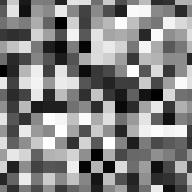
\includegraphics[scale = 0.5]{images/continuousintnoise2d.png}
        \caption{texture 2D obtenu à l'aide de la fonction continue de bruit cohérent}
        \source{http://libnoise.sourceforge.net/noisegen/index.html}
        \end{center}
    \end{figure}
    
    Libnoise part d'une fonction pseudo-aléatoire tel que \textit{rand()} en C++ et prend en paramètres des entiers (ou réel pour la version continue), et renvoyant un entier entre -1 et 1, on appelle cette fonction \textit{integerNoise}.
    
    Le froissement ou plissage de texture (cf figure 2.3) est une imperfection visuelle sur une texture 2D, ces artéfacts forment un pincement à certains endroits. Ils apparaissent car la dérivée de la fonction linéaire aux bornes entières n'est pas définie. Pour éviter les froissements dans la texture, l'interpolation des valeurs entières est indispensable pour avoir des transitions douces entre valeurs de bruit. L'interpolation linéaire est une première version simple mais ne suffit pas à créer un niveau de détail naturel, alors la fonction de bruit cohérent va chercher à utiliser une version non linéaire, couplée à l'interpolation de vecteurs gradients à la place des valeurs entières de bruit. Le vecteur gradient est obtenu avec \textit{integerNoise} qui le sélectionne aléatoirement dans un ensemble de vecteurs précalculés. On utilisera la version 2D de cette fonction, chaque dimension correspond à un paramètre (2 dimensions égal à deux paramètres).
    
    Note : Un ensemble de fonctions de bruits cohérents sera indispensable pour avoir l'essence d'une texture terrain, cette ensemble de fonction se retrouve dans le bruit de Perlin ou de Simplex.
    
     \begin{figure}[h]
        \begin{center}
        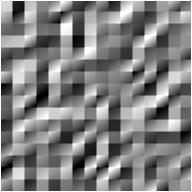
\includegraphics[scale = 0.7]{images/bumpvalue.png}
        \caption{bumpmap "froissée"}
        \source{http://libnoise.sourceforge.net/noisegen/index.html}
        \end{center}
    \end{figure}
    
    \begin{figure}[h]
        \begin{center}
        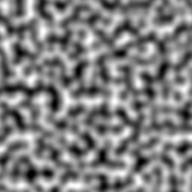
\includegraphics[scale = 0.5]{images/gradientcoherentnoise2d.png}
        \caption{texture 2D avec vecteur gradient}
        \end{center}
    \end{figure}


\vspace*{1cm}


\section{Algorithmes de niveau de détail}

Étant donnée l'importance de l'optimisation pour le rendu temps-réel, il existe de nombreuses approches abordant le problème du stockage et du rendu de HeightMaps. La technique la plus couramment utilisée à l'heure actuelle se base sur des algorithmes de niveaux de détail (Level Of Detail ou LOD) pour subdiviser le maillage de la sphère en fonction de la distance au sol de l'observateur.

Dans un premier temps, nous avons étudié l'article de Filip Strugar \textit{Continuous Distance-Dependent Level of Detail for Rendering HeightMaps}\textbf{\cite{FStrugar}}. Bien que paru en 2010, cet article permet de comprendre plus en détail comment représenter une HeightMap sous forme de quadtree (arbre quaternaire dont les particularités sont expliquées plus bas) et ainsi utiliser cette structure de données pour créer l'algorithme de rendu de HeightMaps CDLOD.

Un quadtree ou arbre quaternaire est un arbre dont chaque noeud dispose au maximum de quatre enfants. Cette représentation est particulièrement utile pour effectuer une subdivision d'un espace en deux dimensions. En effet, une image 2D par exemple peut être partitionnée en quatre quadrants de tailles égales, comprenant chacun l'information de ce quart d'image. Puis, chaque quadrant peut être lui aussi subdivisé en quatre, et ainsi de suite tant que des éléments peuvent être distingués dans celui-ci.

Ici, la HeightMap est représenté par un ensemble de triangle qui constitue le maillage de la surface. 

Le critère sera le nombre maximum de triangles autorisé dans les quadrants finaux. La valeur maximale de triangles dans une feuille est à déterminer par l'équipe de développement, en gardant à l'esprit que plus celle-ci est basse, plus l'arbre sera profond et long à parcourir. De cette manière, chaque quadrilatère continuera à être divisé jusqu'à atteindre cette valeur limite. Un bon moyen de visualiser le processus de création d'un quadtree est l'application interactive \textbf{quadtreevis}\footnote{https://jimkang.com/quadtreevis/}, permettant de visualiser la division de l'image de base ainsi que les noeuds de l'arbre associé.

\subsection{Description de l'algorithme quadtree}
Dans ce projet nous allons utiliser cet algorithme pour pouvoir afficher un niveau de subdivisions du maillage de la surface. En suivant ce tutoriel \footnote{https://www.rastertek.com/tertut05.html}, nous avons trouvé un exemple de code détaillé sur l'algorithme quadtree qui explique comment créer cet arbre.

Pour illustrer le fonctionnement de l'algorithme de l'arbre, nous commençons par un quadruple qui englobe la totalité du terrain. Puis nous le divisons en quatre quadrants et vérifions si chacun de ces quadrants est supérieur à un seuil (nombre de triangles) définit par le groupe. Prenons par exemple $n$ pour le nombre de triangle.  Si le quadrilatère contient plus de n triangles, nous le divisons en quatre quadrilatères de taille égale et nous vérifions à nouveau si chacun des quatre nouveaux quadrilatères contient moins de n triangles ou non. Ainsi de suite. Une fois que chaque quadrilatère de l'arbre entier contient moins de n triangles, nous avons fini de diviser le terrain en sections. Maintenant, pour chaque quadrant, nous déterminons quels triangles lui appartiennent. Nous pouvons représenter cela sous forme de diagramme. Voir figure 2.5. L'algorithme utilise le noeud supérieur de l'arbre pour représenter l'ensemble du terrain. Le deuxième niveau représente les quatre premiers quadrants et ainsi de suite jusqu'à ce que ces derniers répondent au critère de division ou non.

\vspace{0.3cm}

\begin{figure}[h]
    \begin{center}
    \includegraphics[scale = 0.3]{images/qs2.png}
    \caption{étape de division de quadrant entre 2 niveaux de lod}
    \end{center}
\end{figure}

\newpage

Par la suite, il faudra donc créer une bibliothèque permettant la création et la gestion du quadtree, prenant en charge le stockage de la carte et la distinction entre les niveaux de détail. Chaque nœud de l'arbre quadruple sera défini comme suit : position, taille, nombre de triangles et quatre nœuds enfants. La classe aura notamment besoin d'une liste des sommets et du noeud parent pour construire le quadtree de manière récursive. 


\subsection{Description de l'algorithme CDLOD}

Pour appliquer ce principe au stockage de HeightMap, on utilise l'algorithme CDLOD qui pose la contrainte suivante : La profondeur à laquelle nous nous trouvons dans le quadtree correspond toujours au niveau de détail. En d'autres termes, le noeud le plus élevé de l'arbre correspond au niveau de détail le plus bas, et chaque fils comprendra quatre fois plus d'informations (ici des triangles) que les noeuds de l'étage précédent. La figure suivante, tirée de l'article, représente la division d'une HeightMap en 4 niveaux de détail : Du moins détaillé (LOD 3) au plus détaillé (LOD 0).

\vspace{0.3cm}

\begin{figure}[h]
    \begin{center}
    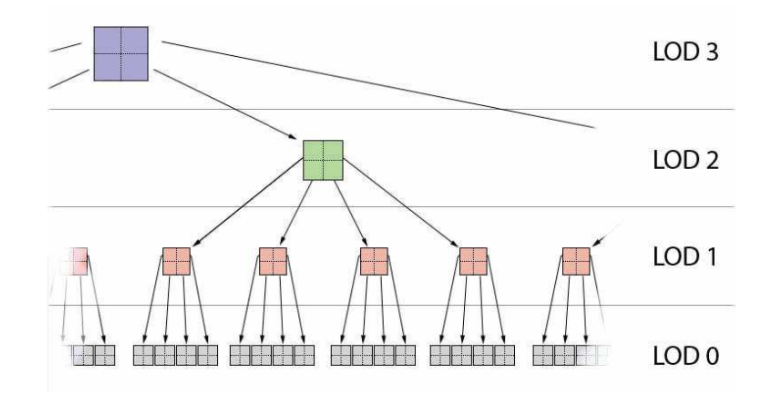
\includegraphics[scale = 0.8]{images/CDLOD1.png}
    \caption{Niveaux de détails sur un quadtree}
    \source{https://github.com/fstrugar/CDLOD/blob/master/cdlod\_paper\_latest.pdf}
    \end{center}
\end{figure}

\vspace{0.5cm}

Ainsi, l'algorithme pourra simplement sélectionner les noeuds correspondant au bon niveau de détail en fonction de la position relative de l'utilisateur par rapport au maillage. Notamment, en utilisant la distance réelle entre l'observateur et les sommets du maillage, il est possible de représenter un nombre de points constant à l'écran et rendre l'algorithme plus prévisible, en théorie. Bien sûr, ces méthodes doivent être adaptées au fait que nous travaillons sur une surface sphérique et non plane, ce qui peut avoir des conséquences sur le calcul de distances et donc sur le rendu final.

\newpage

Selon l'auteur, cette méthode permet de répondre à quelques défaillances des algorithmes de LOD classiques, et met en évidence des besoins qui pourront nous être utiles :

\begin{itemize}
    \item[-] En utilisant la distance réelle et non simplement la latitude/longitude de l'observateur, l'algorithme apporte plus de précision sur les niveaux de détail à afficher. Cet aspect est particulièrement important dans le cas d'une surface sphérique comme c'est le cas ici.
    \item[-] Il permet d'éviter l'apparition d'artefacts graphiques lors des transitions, car le maillage est complètement remplacé avant l'étape de transition.
    \item[-] En terme de performances : Les algorithmes classiques requièrent des calculs additionnels pour afficher des transitions fluides entre les différents niveaux de détail en créant des connexions (sommets) intermédiaires, ce qui n'est pas le cas pour l'algorithme CDLOD.
\end{itemize}


Au final, nous aurons à chaque frame du rendu une carte divisée en niveaux de détails dépendant de la position de l'utilisateur. Sur la figure 2.7, on remarque bien que la division s'affine d'un facteur 2 plus on se rapproche de l'observateur. La zone sombre représente les parties en dehors du champs de vision. 

\vspace{0.3cm}

\begin{figure}[h]
    \begin{center}
    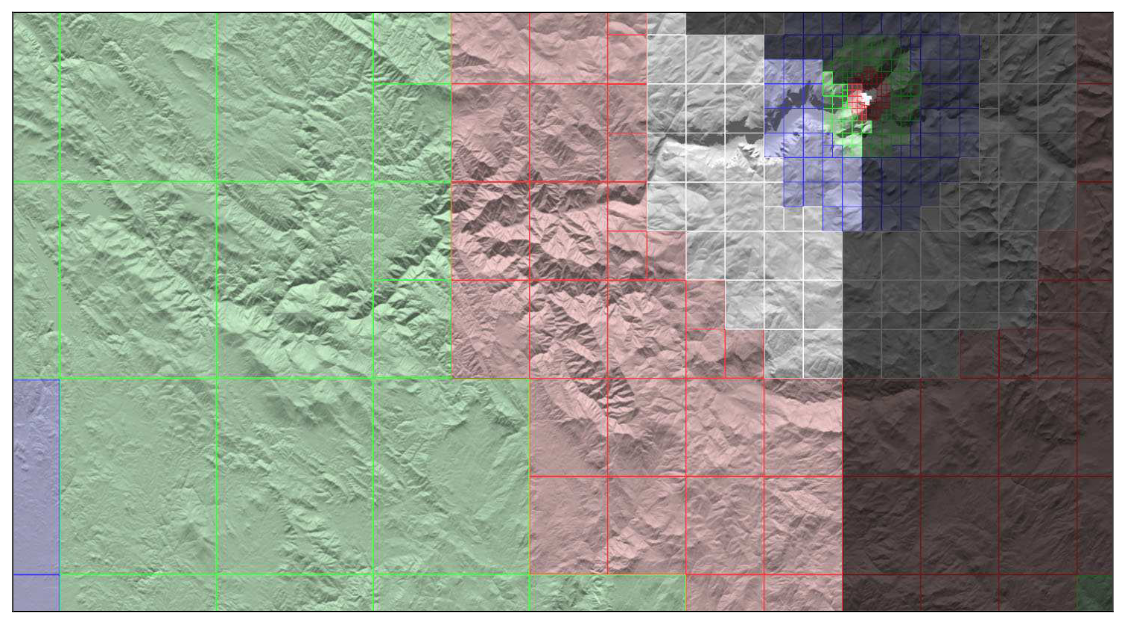
\includegraphics[scale = 0.6]{images/CDLOD2.PNG}
    \caption{carte découpée en LOD}
    \source{https://github.com/fstrugar/CDLOD/blob/master/cdlod\_paper\_latest.pdf}
    \end{center}
\end{figure}


\newpage

\chapter{Les scénarios d'utilisation}
\section{Scénario :}

\begin{enumerate}

\item[\sffamily 1.] Le client lance le fichier exécutable 
\item[\sffamily 2.] Un explorateur de fichier s'ouvre, demandant à l'utilisateur de spécifier l'emplacement d'une HeightMap. Le logiciel va alors stocker cette HeightMap sous forme de quadtree.
\item[\sffamily 3.] Une fenêtre graphique s'ouvre affichant le rendu placé sur le centre de la heighmap.
\item[\sffamily 4.] Le client dezoom via la molette de sa souris.
\item[\sffamily 5.] Le client se déplace sur la surface à l'aide des flèches de son clavier. 
\item[\sffamily 6.] Le client applique une rotation sur la planète en appuyant sur la touche R.
\item[\sffamily 7.] L'utilisateur choisit de changer de HeightMap en appuyant sur la touche C.
\item[\sffamily 8.] L'utilisateur active le maillage en appuyant sur la touche M.
\item[\sffamily 9.] Le client choisit d'afficher des informations sur le programme en appuyant sur la touche H.
\item[\sffamily 10.] L'utilisateur met le programme en pause en appuyant sur P.
\item[\sffamily 11.] Le client quitte le logiciel en appuyant sur Q.



\end{enumerate}

\section{Extensions :}

\begin{enumerate}

\item[\sffamily 1a.] La configuration de l'appareil du client ne permet pas de  faire fonctionner notre logiciel.
\begin{itemize}
    \item Un message d'erreur s'affiche et le logiciel ne s'exécute pas.
\end{itemize}
\item[\sffamily 2a.] L'utilisateur ferme l'explorateur de fichier
\begin{itemize}
    \item Le logiciel se ferme
\end{itemize}
\item[\sffamily 2b.] Le client utilise le logiciel avec un fichier ne correspondant pas à une HeightMap ou pas compatible avec notre implémentation.
\begin{itemize}
    \item Un message d'erreur s'affiche et le logiciel se ferme.
\end{itemize}

\end{enumerate}
\chapter{Description des besoins}

\section{Besoins Fonctionnels}

\begin{enumerate}
    \item \textbf{Lecture des HeightMaps en entrée} : De manière générale, les HeightMaps sont stockées dans des formats d'images standard car elles représentent une structure de valeurs en 2D, chaque pixel contenant la hauteur du terrain en ce point. Noiseutils, l'utilitaire pour sauvegarder les HeightMaps en image, ne supporte que l'extension .bmp. Il serait tout de même possible d'ajouter d'autres extensions, soit en ajoutant une classe utilitaire faite maison, soit en utilisant une autre bibliothèque pour sauvegarder notre HeightMap en image 2D.
    
    \item \textbf{génération de HeightMap}
    \begin{enumerate}
        \item générer une carte de hauteur quelconque.
        \item spécifier la taille de la carte en pixels.
        \item générer une carte 2D sphérique : les bords gauches et droits se rejoignent de manière harmonieuse, et une distorsion se produit au niveau des pôles.
        \item pouvoir influencer le détail de la carte, son nombre d'octave pour une quantité de détails accrue mais plus petits, sa fréquence pour plus de particularités sur le terrain, sa persistance pour un terrain plus ou moins lisse.
        \item générer aléatoirement une carte, donner uniquement la taille et le nom de l'image créée.
        \item Nommer la carte
        \item ajouter un gradient couleur pour faire une distinction entre zones en altitudes et zones au niveau 0. Permet d'avoir une figuration plus agréable.
        \item complexifier le terrain en ajoutant des "noise modules" disponibles sur libnoise, laisser le choix à l'utilisateur d'ajouter des vallées, montagnes, lacs, terrains sableux, des turbulences pour un peu de réalisme etc.
    \end{enumerate}
    
    \item \textbf{Algorithme CDLOD} :
    \begin{enumerate}
        \item La première étape de l'algorithme est le stockage de la HeightMap sous forme de quadtree. Cette étape implique la création d'une structure maison pour un quadtree. Celle-ci devra permettre au minimum la création et la suppression d'un arbre, l'ajout et la suppression de noeuds ainsi qu'une méthode de parcours de l'arbre.
        \item Dans un second temps, nous devons effectuer la sélection des noeuds du quadtree pour le rendu. Cette action est effectuée à chaque fois que l'observateur se déplace dans la scène, et donc possiblement à chaque frame. Pour savoir quels noeuds sont sélectionnés, les distances couvertes par chaque niveau de LOD sont pré-calculées (cf Partie 2.2 : \textit{Algorithmes de niveau de détail}). A chaque fois qu'un mouvement est détecté, l'algorithme recherche les noeuds représentant les parties du terrain actuellement visibles et le niveau de détail avec lequel elles doivent être tracées.
        \item Enfin, chaque noeud sélectionné doit être stocké dans une structure de données temporaire qui doit contenir sa position dans la scène, sa taille et son niveau de détail. D'autres informations peuvent y être ajoutées si elles sont nécessaires au rendu graphique.
    \end{enumerate}

    \item \textbf{Visualisation OpenGL} :
    \begin{enumerate}
        \item \textbf{Fenêtre de visualisation} : 
            Création par programmation d'une fenêtre de visualisation qui interagit avec un objet de HeightMap. La première étape pour utiliser OpenGL est de créer un context et généralement une fenêtre associée capable d'afficher un rendu OpenGL. Ces deux tâches seront effectuées par la bibliothèque GLFW.
            
            \begin{itemize}
                \item \textbf{GLFW} est une bibliothèque Open Source multiplateforme pour le développement OpenGL sur le bureau. Il fournit une API simple pour créer des fenêtres, des contextes et des surfaces, recevoir des entrées et des événements.
            \end{itemize}
            \begin{figure}[h]
                \centering
                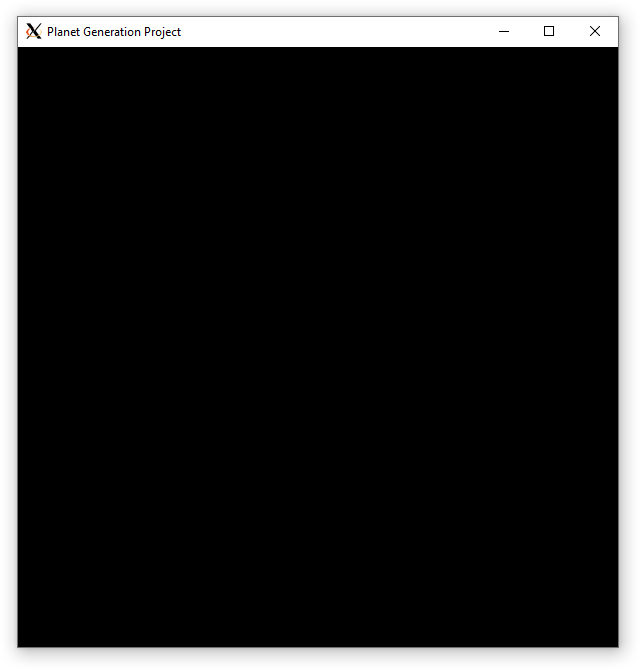
\includegraphics[scale = 0.5]{images/Fenetre_de_visualisation.png}
                \caption{Exemple de fenêtre de visualisation. WSL2. XLaunch.}
            \end{figure}
                \newpage
        \item \textbf{Création de la fonctionnalité nécessaire et intégration de l'existant pour un fonctionnement pratique de base} :
        Dans cette partie, nous allons utiliser deux bibliothèques : Eigen et Glbinding. 
        \begin{itemize}
            \item \textbf{Eigen} est une bibliothèque C++ d'algèbre linéaire. Elle sera utilisée pour la représentation et manipulation de matrices, vecteurs, transformations géométriques et résolution de systèmes d'équations.
            \item \textbf{Glbinding} exploite des fonctionnalités C++ 11 telles que les classes enum, les lambdas et les modèles variadiques. Tous les symboles OpenGL sont de véritables fonctions et variables. Il fournit des paramètres de sécurité de type, des en-têtes d'API par fonctionnalité, une résolution de fonction paresseuse, une prise en charge multi-contextes et multi-threads, des méta-informations sur la liaison OpenGL générée et le runtime OpenGL, ainsi que des outils et des exemples.
        \end{itemize}
        \item \textbf{Initialisation de la caméra} : 
        La portée de vue de la caméra et sa position décident des nœuds à dessiner et de la profondeur de la cascade des nœuds. Les nœuds les plus proches de la caméra sont en cascade jusqu'aux nœuds feuilles, dessinant une géométrie plus dense. La fonctionnalité de la caméra consiste à déplacer l'utilisateur sur une zone ou à modifier la distance de rendu d'un objet à l'aide des boutons. 
        \begin{itemize}
            \item PAGE UP : Déplacer vers le haut
            \item PAGE DOWN : Déplacer vers le bas
            \item KEY UP : Tourner la caméra vers le haut
            \item KEY DOWN : Tourner la caméra vers le bas
            \item KEY LEFT : Tourner la caméra à gauche
            \item KEY RIGHT : Tourner la caméra à droite
            \item KEY E : Avancer
            \item KEY D : Reculer
            \item KEY S : Déplacer vers la gauche
            \item KEY F : Déplacer vers la droite
            \item KEY W : Définir le mode wireframe
        \end{itemize}
        
        \begin{figure}[h]
            \centering
            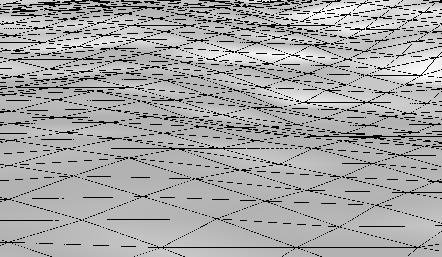
\includegraphics[scale = 0.7]{images/mesh_edges.png}
            \caption{Exemple de mesh edges.}
            \source{https://github.com/drecuk/QuadtreeTerrain}
        \end{figure}
         \begin{figure}[h]
            \centering
            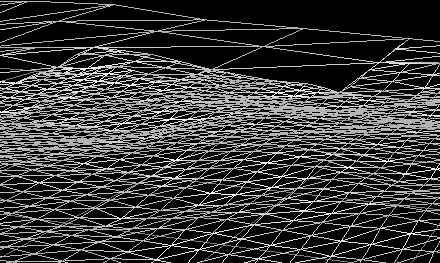
\includegraphics[scale = 0.7]{images/view_quadtree.png}
            \caption{Exemple de visualisation d'un Quadtree en mode wireframe}
            \source{https://github.com/drecuk/QuadtreeTerrain}
        \end{figure}
        
           \newpage
        \item \textbf{Implémentation logicielle de CDLOD} :
        La supclasse crée et maintient une structure quadtree. Chaque noeud de cette structure est décrit par la structure de noeud. Ceci décrit les points à partir desquels les quads OpenGL sont construits (surface du terrain). Chaque nœud a 3 x 3 sommets, que notre constructeur utilise pour dessiner des triangles.
        \item \textbf{Chargement du fichier RAW} :
        Le remplissage de la structure de données avec les données RAW bitmap de 8 bits pour chaque élément du tableau. Ce sont ces données qui seront utilisées pour visualiser le HeightMap.

    \end{enumerate}
        \newpage
    \item \textbf{Rendu planétaire} : Le processus de rendu planétaire nécéssite un objet géométrique de base comme un cube ou octahedron, qui sera ensuite subdivisé à l'aide de la distance caméra - sommets visibles. Des algorithmes comme LOD ou CDLOD détermineront les détails à afficher. Aussi il sera indispensable de mêler notre carte de hauteur à la sphère générée, pour élever ou réduire le terrain à différents endroits. On devrait pouvoir utiliser autant que possible le GPU pour ce genre d'opérations avec plusieurs centaines de triangles affichés en même temps. Le terrain invisible (de l'autre côté de la face observée par la caméra) ne doivent pas être rendu (backface culling & frustum culling).
    \begin{enumerate}
        \item subdiviser un cube et afficher une sphère
        \item appliquer l'algorithme LOD sur ce cube et employer le bon niveau de subdivision en fonction de la distance par rapport à la caméra. Respecter une distribution géométrique constante dans l'idéal, c'est à dire que le nombre de triangle à afficher reste toujours le même, qu'importe la proximité de la caméra.
        \item ajouter une carte de hauteur pour modifier l'altitude, le terrain et le lissage de la sphère.
        \item Activer le culling pour n'afficher que ce qui est visible par l'utilisateur, et éviter une perte de calcul et de temps. 
    \end{enumerate}
    
    
\end{enumerate}

\vspace{0.3cm}

\section{Besoins Non-Fonctionnels}

\textbf{Taille des données en mémoire} : L'implémentation pratique d'un logiciel de rendu de terrain doit tenir compte de la taille de ce dernier. Ici, il y a deux facteurs principaux à prendre en compte :
\begin{enumerate}
    \item \textbf{Les données de terrain} : Pour ne pas garder la totalité des données de la HeightMap en mémoire, celle-ci peut-être divisée en blocks représentants les morceaux de terrain potentiellement visibles par l'observateur. Au lieu d'envoyer toutes les informations au GPU, on trie les éléments visibles et invisibles pour ne tracer que les éléments visibles. Grâce à cette technique, on gagne du temps de calcul GPU. Ces fragments peuvent être transmis sous forme de data-stream pendant le rendu. Cette méthode est d'autant plus efficace que l'algorithme CDLOD effectue déjà une sélection des blocks lors du calcul de LOD. 
    \item \textbf{Les données du quadtree} : Plus volumineux encore, les noeuds du quadtree contiennent des détails tels que la taille, la position, les voisins du noeud, etc... beaucoup d'informations qui peuvent être superflues pour l'étape de rendu. La version StreamingCDLOD de l'algorithme présenté dans le chapitre 2.2 évite ce problème en ne gardant que les valeurs minimales et maximales de la surface couverte par le noeud, qui sont stockées dans une matrice 2x2 pour chaque noeud. Le reste des données est automatiquement généré lors du parcours du quadtree.
    \item \textbf{Performance}: On exige que le temps de rendu soit acceptable par un utilisateur lambda, soit avec un minimum de 25 image par seconde pour avoir un rendu cinématique. L'intéractivité  n'est pas au centre du projet, ce pourquoi le rendu cinéma peut-être apprécié.
    \item \textbf{Passage à l'échelle} : Lors de la création du quadtree ou dans la phase de rendu, s'assurer que le programme puisse gérer des HeightMaps très grandes et très détaillées.
    \item \textbf{HeightMap}
    \begin{enumerate}
        \item génère infailliblement une image 2D
        \item génération instantanée, de l'ordre d'une milliseconde
        \item est utilisable dès sa création, peut-être utilisée pour ajouter la suite du terrain 3D sur le tas sans chargement (génération procédurale)
    \end{enumerate}
    \item \textbf{Visualisation OpenGL} :
    \begin{enumerate}
        \item \textbf{Performance:}
        \begin{enumerate}
            \item Le temps de traitement du programme ne dépasse pas quelques minutes.
            \item Garder un affichage fluide de rendu de HeightMap.
        \end{enumerate}
            \item \textbf{Contraintes et difficulté techniques:}
            \begin{enumerate}
                \item Surface sphérique. L'ordinateur doit générer un maillage de base convexe pendant la génération du terrain.
                \item Utiliser un maillage de triangle équilatéraux plutôt que d'autres polygones.
            \end{enumerate}
        \item \textbf{Portabilité:}
        \begin{enumerate}
            \item Utiliser une machine contenant une carte graphique avec une version d'openGL de préférence openGL 3.3.
            \item Ajouter le contrôle de la molette de la souris au lieu de boutons, pour un contrôle plus facile de la caméra.
        \end{enumerate}
        \item \textbf{Contraintes d'affichage:}
        \begin{enumerate}
            \item Faire des tests pour pouvoir afficher un nombre conséquents de triangles.
            \item Récupérer la taille totale et restante de la mémoire du GPU avec GL NVX gpu memory info.
        \end{enumerate}
    \end{enumerate}
\end{enumerate}

Enfin, il est possible de compresser d'une part les HeightMaps, et d'autre part les données des noeuds les plus détaillés du quadtree, en stockant les valeurs de la matrice min/max du noeud dans l'espace inutilisé de la matrice du noeud parent avec une faible perte de précision.

\newpage

\chapter{Prototypes et choix techniques}

\section{Language de programmation}

Au vu de l'analyse de l'existant et des contraintes du projet, nous avons choisi d'utiliser le langage C++ pour développer nottre application. En effet, une grande partie des projets et des librairies traitant du sujet utilisent le C++, notamment pour des raisons d'efficacité de gestion de la mémoire qui est un point crucial du projet.

De même, l'utilisation de la bibliothèque OpenGL sera grandement facilitée car nous avons déjà tous une certaine expérience à l'utiliser avec ce langage. Pour s'assurer que notre programme puisse fonctionner sur différents systèmes et configurations, nous utiliserons OpenGL 3.3.

\section{Implémentation du module CDLOD}

Pour commencer à réaliser la transformation des HeightMaps en quadtrees, nous sommes partis de HeightMaps simples préconstruites et distribuées sous license libre.

\begin{figure}[h]
    \centering
    \includegraphics[scale = 0.7]{images/simple_HeightMap_1025.PNG}
    \caption{HeightMap plane 1025x1025, PNG}
    \source{https://www.motionforgepictures.com/height-maps}
\end{figure}

\newpage

La première contrainte apparaissant ici est celle du format des HeightMaps. En effet, les cartes que nous avons trouvé ne sont pas en .RAW comme nous le pensions mais dans différents formats image tels que PNG, JPG ou encore EXR. Nous avons donc commencé par utiliser la librairie Magick++, permettant d'utiliser les fonctions de l'outil ImageMagick. Celà nous permettra d'ouvrir simplement des images dans différents formats, de parcourir les données et extraire les valeur des pixels qui nous intéressent. Théoriquement, la bibliothèque libnoise pourra à terme remplacer ces cartes génériques et nous fournir directement une structure de valeurs utilisables par l'algorithme.

Comme nous l'avons expliqué dans la partie 2.2, l'algorithme de création du quadtree se base sur la position des sommets sur un plan 2D. Si le nombre de sommets présents dans le noeud est supérieur à notre valeur limite, alors celui-ci est découpé en quatre noeuds enfants de la manière suivante (figure 6.2).

\begin{figure}[h]
    \centering
    \includegraphics[scale = 0.35]{images/CDLOD_Childnode.png}
    \caption{définition du premier noeud enfant}
\end{figure}

Tant que la condition $currentNode.leaf == true$ n'est pas respectée, cette récursion se poursuit. Pour imager ce processus, nous pouvons nous appuyer sur la figure 6.3, tirée de l'article \textit{Quadtree Procedural Terrain}\cite{ECh'ng}, qui explique la division d'un quadrant en quatre enfants.

\newpage

\begin{figure}[h]
    \begin{center}
    \includegraphics[scale = 0.25]{images/Quadtree_construction.png}
    \caption{Découpage du noeud racine (512x512) en quatre noeuds enfant (256x256)}
    \source{https://github.com/drecuk/QuadtreeTerrain/blob/master/QuadtreeTerrain.pdf}
    \end{center}
\end{figure}

\vspace{0.3cm}

Nous remarquons ainsi que chaque fils représente une surface quatre fois moins importante que celle du père, mais contient toujours autant de faces et de sommets, ce qui signifie que la surface sera plus détaillée si ce noeud est sélectionné.

Finalement, chacun des sommets représentés dans un noeud se voit attribué une valeur de hauteur, fournie par la HeightMap. Lors du rendu, les noeuds des sommets sélectionnés seront donc affichés à l'endroit défini par le quadtree, et à la hauteur définie par la carte.

\section{Module frustum culling}

Nous avons aussi essayé d'implémenter le processus de "frustum culling" pour réduire le nombre de sommets à tracer. Nous avons tout d'abord crée une autre branche que nous avons déposé sur notre gitlab pour pouvoir se consacrer uniquement sur cette étape et la fusionner avec la branch "main" par la suite.
Cette technique a pour but d'afficher uniquement les éléments visibles de la scène en se basant sur le cône de vision de la caméra. Celui-ci délimité par 6 plans qui forment la pyramide de vision.  Ainsi, tout ce qui est dans la zone est affiché et les éléments en dehors ne sont pas calculés. L'avantage majeur est de réduire la quantité de calculs nécessaires du processeur graphique.

\begin{figure}[h]
            \centering
            \includegraphics[scale = 4]{images/VisualCameraFrustum.png}
            \caption{pyramide de vision}
            \source{https://learnopengl.com/Guest-Articles/2021/Scene/Frustum-Culling}
        \end{figure}
\newpage   
Les plans sont construits avec un point et une normale. Le principe du frustum culling dans notre cas repose sur une fonction essentielle qui est de déterminer si la position de chaque sommet de la surface du maillage est dans la pyramide de vision délimitée par les 6 plans ou non. Cette fonction va donc utiliser le produit scalaire. Le produit scalaire nous permet d'obtenir la projection d'un vecteur sur un autre. 
On va donc faire une opération qui va utiliser ce calcul. Si le sommet est à l'intérieur des six plans, elle renvoie vrai, sinon la fonction renvoie faux.
Ce principe est utilisé dans la fonction createFrustum du fichier mesh.cpp qui va donc créer les sommets et les faces pour le frustum et l'envoyer au GPU à l'aide de updateVBO(). Ensuite, cette fonction est utilisé dans le fichier Viewer.cpp. Au niveau du rendu de la heigthmap losqu'on appuie sur la touche "c" nous voulons que la partie des sommets invisibles ne soient pas affichée à l'écran mais cela ne fonctionne pas correctement. Dans notre cas nous voyons soit toute la surface affichée soit rien d'affiché. 

\newpage

\chapter{Architecture de l'application}
\begin{figure}[h]
    \centering
    \includegraphics[width=1.1\textwidth]{images/Diagramme_classes.png}
    \caption{Diagramme de classes de l'application en l'état}
\end{figure}
\section{Un point sur ce qui a été réalisé}
Toute les classes présentes dans le diagramme sont présentes dans le projet, la seule différence portant sur les relation entre les classes. On observe une aggrégation entre MapLoader et Terrain et TrackBall et OpenGLViewer. Pour les 2 relations dans l'application ce sont de simples compositions. 

Pour MapLoader on pourrait imaginer que l'application puisse lire des HeightMap ou les générer ainsi on utiliserait le pattern Singleton sur cette classe et pour tout notre projet on aurait un point d'entrée commun pour toute les classes

Pour TrackBall il serait tout à fait envisageable de l'abstraire et que plus tard le DirectXViewer et l'OpenGLViewer aient tout les deux leurs propres implémentations.

\section{Présentation des patterns implémentés}
Sur le diagramme on observe 2 pattern, un premier avec l'implémentation de QuadTree depuis TerrainGeneration, c'est le pattern Builder. Ici l'utilisateur qui est représenter par la classe Terrain va instancier le QuadTree via la méthode compile(), Quadtree va implémenter cette méthode avec sa spécification ainsi on pourra ajouter plus tard une autre méthode que QuadTree (comprendre CDLOD). Enfin l'utilisateur va pouvoir récupèrer un vecteur de QTNode grâce à getResult().

On observe aussi un autre pattern avec ViewerAbstract et OpenGLViewer, nous voulions au départ implémenter le pattern Facade, au final nous avons décidé de seulement abstraire la classe Visualisation. En effet la motivation principale était de pouvoir ajouter par la suite un autre outil de visualisation (DirectX par exemple), mais lorsque qu'on implémente l'architecture nous sommes influencer par les outils utilisés (ici OpenGL), ainsi il était difficile d'implémenter ce pattern tout en gardant à l'esprit qu'il fallait qu'il soit prêt par la suite pour un autre moteur 3D. Donc nous avons simplement abstrait Viewer.

\section{Diagramme de séquence}
\begin{figure}[h]
    \centering
    \includegraphics[width=1\textwidth]{images/Diagramme_Sequence.PNG}
    \caption{Diagramme de séquence de l'application en l'état}
\end{figure}
Point important pour le diagramme de séquence ci-dessus : il représente une séquence à un moment avancer du lancement de l'application, c'est à dire que le QuadTree est considérer comme déjà générer et afficher.

\chapter{Fonctionnement}

\section{Module CDLOD}

Dans cette partie nous allons expliquer les résultats que nous avons obtenu lorsque nous lançons notre algorithme. Tout d'abord il faut expliquer que nous n'avons pas fait le continuous de CDLOD qui correspond à la transition fluide entre 2 niveaux de détails et notamment le calcul de l'affichage de plusieurs niveaux de détails sur une même surface. Nous nous sommes attardés sur le bon fonctionnement du rendu d'une surface qui contient qu'un seul niveau de détail à la fois. 
Mais avant cela, nous avons tout d'abord réussi à afficher une heigthmap sans quadtree et nous pouvons aussi nous déplacer partout ou on le souhaite sur cette surface de maillage. Voici le rendu suivant:

\begin{figure}[h]
            \centering
            \includegraphics[scale = 0.3]{images/rendu.png}
            \caption{affichage sans quadtree}
        \end{figure}


Dorénavant, voici les résultats qu'on obtient pour le LOD 4, 5 et 6.

\begin{figure}[h]
            \centering
            \includegraphics[scale = 0.1]{images/LOD4.png}
            \caption{affichage du lod 4}
        \end{figure}
        
\begin{figure}[h]
            \centering
            \includegraphics[scale = 0.1]{images/LOD5.png}
            \caption{affichage du lod 5}
        \end{figure}
        
\begin{figure}[h]
            \centering
            \includegraphics[scale = 0.1]{images/LOD6.png}
            \caption{affichage du lod 6}
        \end{figure}
\newpage

Nous pouvons voir que la position de chaque sommet n'est pas placée correctement sur la carte. Cela est du sûrement à un problème dans notre code qu'on n'arrive pas bien à repérer car nous n'avons pas réussi à résoudre ce problème. Nous pouvons quand même voir une différence entre chaque LOD, que ce soit au nombre de sommet et de triangles. En effet, on peut apercevoir qu'il y a plus de triangles lorsqu'on augmente le niveau de détail avec un effet plus condensé. 

\chapter{Tests}

\section{Test Génération des HeightMaps}

\subsection{Test Generate Between}
\begin{enumerate}
    \item Description : fonction assistante pour la génération aléatoire de la carte et de boites englobantes (voir les tests plus bas). Ce test s'assure que la valeur retournée est bien bornée entre deux variables élues.
    \item Cas de test :
    \begin{itemize}
        \item valeur aléatoire entre 0 et 1 : résultat attendu : succès.
        \item valeur aléatoire entre -100 et 0 : résultat attendu : succès.
        \item valeur réelle aléatoire entre 1.2 et 1.8 : résultat attendu : succès.
        \item valeur réelle négative aléatoire entre -10000.5 et -10000 : résultat attendu :succès.
    \end{itemize}
    \item déroulement du test : On utilise pas de stratégie particulière. 
    \emph{CPP\_UNIT\_ASSERT} est notre meilleur ami dans ce cas de test unitaire.
    \item résultats : les tests sont les résultats attendus.
\end{enumerate}


\subsection{Test Bounding Box}
\begin{enumerate}
    \item Description : Le builder génère les valeurs de bruits cohérents à partir des valeurs contenues dans un rectangle définie, appelée bounding box dans notre programme. Les coordonnées de la boite sont à définir avant de générer la HeightMap. Cette boite sert aussi au tiling, c'est à dire à définir une suite direct à la HeightMap sur l'un de ses quatres points cardinaux. Ce test s'assure de la bonne définition de la boite.
    \item Cas de test : 
    \begin{itemize}
        \item rectangle quelconque lowerX = 0, UpperX = 2, LowerZ = 1, UpperZ = 8. Résultat attendu : succès
        \item rectangle dont toutes les coordonnées sont les mêmes (un point). Résultat attendu : échec
        \item rectangle mal positionné (coordonées d'une ligne). Résultat attendu : échec
        \item rectangle avec lowerX supérieur à UpperX. Résulat attendu : échec
        \item rectangle avec lowerZ supérieur à UpperZ. Résultat attendu : échec
        \item rectangle avec des réels. Résulat attendu : succès
        \item rectangle dans les valeurs négatives. Résultat attendu : succès
        \item rectangle à frontière entre positif et négatif. Résultat attendu : succès
    \end{itemize} 
    \item déroulement du test : Pas de technique ni d'algorithmes particuliers utilisés, nous utilisons \emp{CPP\_UNIT} pour réaliser nos tests unitaires. Sur ce test, nous récupérons le builder et nous vérifions après l'appel de \underline{GeneratePlanarHeightMap} que les valeurs passées à la boite sont équivalentes. Il y a aussi des tests négatifs qui sont sensés lever des exceptions.
    \item résultats : Les tests ont les résultats attendus.
\end{enumerate}

\subsection{Test de la taille des HeightMaps}
\begin{enumerate}
    \item Description : Générer une carte dont la taille est indiquée par l'utilisateur. On s'assure simplement du bon fonctionnement de la fonction \underline{GeneratePlanarHeightMap}. L'objectif est de commencer à chercher les limites de la bibliothèque libnoise, jusqu'où peut-elle aller ? A ce stade des tests il n'y a pas de sauvegarde dans un fichier, puisque la fonction sauvegarder n'a pas encore été testée, mais elle nécessite celle-ci.
    \item Cas de test
    \begin{itemize}
        \item HeightMap quelconque de taille 150x150. Résultat attendu : succès
        \item HeightMap négatives avec des tailles 0x0, -5x5, -1x0 et 0x40, hors du domaine tolérée. Résultats attendus : échec.
        \item HeightMap gigantesque. Résultat attendu : succès.
        \item HeightMap avec taille maximale autorisée. Résultat attendu : succès.
    \end{itemize}
    \item Déroulement du test : Le test s'effectue aussi avec \emp{CPP\_UNIT} et ses assertions. Nous récupérons le builder de la HeightMap à partir d'un getter, et celui-ci possède les attributs de hateur et largeur passée à l'utilisateur, cela valide nos test sensés fonctionner. Pas de stratégie de test particulière appliquée.
    \item Résultats : Les trois premiers items sont tous attendus. Pour le troisième test, il a fallu patienter une bonne minute. Pour le dernier test, il ne se termine pas dans les temps que l'on juge correct (plus d'une minute), aussi nous avons décidé d'avorter ce test là.
\end{enumerate}

\subsection{Test de sauvegarde de la HeightMap}
\begin{enumerate}
    \item Description : Vérifier la création d'un fichier image au format bmp dans le dossier \textbf{textures}. S'assurer de la robustesse de la fonction de sauvegarde pour qu'elle ne plante pas au moindre faux pas. La fonction \underline{Save} transforme le tableau de valeurs de bruit de Perlin obtenue avec le builder de libnoise en image 2D, elle est appelée après \underline{GeneratePlanarHeightMap}.
    \item Cas de test :
    \begin{itemize}
        \item fichier en .raw. Résultat attendu : succès.
        \item fichier en .png. Résultat attendu : succès.
        \item fichier en .jpg. Résultat attendu : succès.
        \item fichier en .jpeg. Résultat attendu : succès.
        \item fichier en .bmp. Résultat attendu : succès.
    \end{itemize}
    \item Déroulement du test : pour réaliser ce tests, il était nécéssaire de voir si l'enregistrement avait eu lieu, donc de pouvoir ouvrir le fichier venant d'être enregistré. Pour cela Magick++ a été une fois de plus utile, jugeant de ses bonnes fonctionnalités, nous avons pu vérifier que la lecture du fichier ne pose aucun problème. Le test en profite pour vérifier si la largeur et la hauteur de l'image ainsi que l'extension sont exactes.
    \item Résultats : presque tous sont des échecs, rien d'étonnant quand on apprend que libnoise a une classe writerbmp et uniquement cette classe pour enregistrer les images en .bmp. Ce qui portait à confusion c'était le fait de pouvoir ajouter une extension sans que libnoise ne soulève une exception. Grâce à ce test nous avons donc corriger un bug possible dans l'utilisation de notre application. Nous nous contentons d'une seule extension pour les HeightMaps, mais cela pourra être corrigé plus tard comme dit plus haut. Seul un test a été concluant, les autres ont été revus et passés en tests négatifs.
\end{enumerate}

\subsection{Test Benchmark des tailles de HeightMaps}
\begin{enumerate}
    \item Description : Ce test va permettre d'apporter plus de précision sur les limites possibles de notre application, et surtout quels pourraient être les tailles optimales pour une HeightMap dont le rapport taille-temps n'a pas d'impact sur l'utilisation en temps réel. Il permet aussi de vérifier la robustesse de la bibliothèque libnoise puisqu'on va générer 20 HeightMaps à la suite sans interruptions.
    \item Cas de test :
    \begin{itemize}
        \item 20 HeightMaps avec taille évolutive, dont toutes sont générées sans problèmes, mais pas sauvegardées, elles restent en mémoire. Résultat attendu : succès
    \end{itemize}
    \item Déroulement du test : La stratégie adoptée consiste à itérer sur une boucle pour créer 20 HeightMaps dont la taille en hauteur et largeur augmente de 100 pixels à chaque pas de boucle. Pour tracer le déroulement, nous écrivons dans un fichier texte la taille et la durée de génération associée.
    \item Résultats : Il faut souligner la robustesse de la bibliothèque libnoise qui malgré les 30 seconde sans pouvoir reprendre le terminal, délivrent des résultats sans problèmes, et génèrent des images jusqu'à 2000x2000 en 4 secondes. Pas besoin de pousser très loin l'analyse pour détecter les tailles idéales sur lesquellles nous devrions baser nos modèles de HeightMaps, et cela voudrait dire limiter l'utilisateur lambda à que quelques tailles, au risque de le voir s'impatienter et fermer l'application sans terminaison propre. Sur la figure ci-dessous, plus la taille augmente plus le temps de génération augmente, la frontière consiste à sélectionner une taille au dessus de laquelle il n'est pas recommandé de passer si on souhaite un framerate correct d'au moins 25 images par secondes. Si on prend seulement en compte la génération de la HeightMap, qui se fait en amont du quadtree, on peut se permettre de prendre jusqu'à une seconde de génération, soit une taille de 1000x1000 pixels, sachant qu'il est possible de faire de grandes textures avec des petites tailles de HeightMaps tel que 256x256. La frontière est un point de discussion assez conflictuel.
    
    \begin{figure}[h]
    \begin{center}
    \includegraphics[scale = 1]{images/benchmark_size.jpg}
    \caption{Illustration du benchmark sur les tailles testées}
    \end{center}
\end{figure}
    
\end{enumerate}

\subsection{Test Benchmark Stress}
\begin{enumerate}
    \item Description : Ce test, tout comme le test précédent, nous sert de référence pour situer le potentiel de notre application, pour confirmer notre code et prendre confiance sur celui-ci, pouvoir présenter notre assurance à l'utilisateur en présentant des résultats tangibles. Il consiste à générer un nombre important de HeightMaps avec une taille qui ne prend pas plus d'un tiers de seconde à être générée.
    \item Cas de test
    \begin{itemize}
        \item 100 HeightMaps 500x500
    \end{itemize}
    \item Déroulement du test : On effectue 100 tours de boucles qui génèrent 100 HeightMaps de tailles fixes, elles sont vérifiées avec \emph{CPP\_UNIT} lors de la création, et tout comme l'autre test, nous écrivons dans un fichier la durée de chaque tour de boucle. La boite englobante est la seule variable changeante puisqu'elle est générée aléatoirement entre -100 et 100 pour x et pour z. On va pouvoir avoir un aperçu de l'influence de cette boite sur les performances.
    \item Résultat : Une partie des résultats est disponible ci-dessous, une image parle toujours mieux que des mots. Nous n'avons pas eu le temps de traiter les données bruts du test et en faire quelques statistiques, mais à vu d'oeil, nous pouvons être certains que la taille de la boite englobante a un effet sur le poids de calcul. Il aurait été intéressant de calculer pour chaque boite son aire, et faire tourner ce test sur plusieurs tailles pour confirmer cette hypothèse. On peut voir que l'algorithme tient ses promesses et génèrent 100 HeightMaps de taille 500x500 sans problèmes en moins de 300 millisecondes. Cette information nous rassure sur notre architecture et notre code, et il va pouvoir être utilisé peut-être pour plus tard pour générer à la volée des cartes aléatoires sans perte de gain énorme, mais cela reste encore du prototypage.
    
    \begin{figure}[h]
    \begin{center}
    \includegraphics[scale = 0.8]{images/benchmark_stress.jpg}
    \caption{Illustration du benchmark obtenu lors du test de stress}
    \end{center}
\end{figure}
    
\end{enumerate}


\subsection{Test avec une HeightMap existante}
\begin{enumerate}
    \item Description : C'est un test avec existant, libnoise génère la même HeightMap que le générateur, et il suffit de comparer les deux et instaurer une couche de confiance supplémentaire sur notre générateur.
    \item Cas de test :
    \begin{itemize}
        \item 2 HeightMaps générées, l'une avec libnoise l'autre avec le générateur, tous les pixels de l'image sont comparés. Résultat attendu : succès
    \end{itemize}
    \item Déroulement : A l'aide de Magick++, on parcours en même temps les deux images générées, et on assert via \emph{CPP\_UNIT}.
    \item Résultat : Le résultat est concluant, les images sont les mêmes lorsqu'on modifie aucun paramètre par défaut.
\end{enumerate}

\subsection{Test SetOctave}
\begin{enumerate}
    \item Description : Teste la définition du nombre d'octaves qui servent à complexifier la carte, augmentent les détails de la carte. 
    \item Cas de test :
    \begin{itemize}
        \item Octave négatif. Résultat attendu : échec.
        \item Octave 0. Résultat attendu : échec.
        \item Octave au dessus du domaine (31 octaves). Résultat attendu : échec.
        \item 8 Octaves. Résultat attendu : succès.
    \end{itemize}
    \item Déroulement : Parcours des deux images créées avec libnoise et le générateur, utilisation de Magick++ pour comparer les pixels.
    \item Résultat : Les résultats sont concluants, mais unique dans le sens où à nombre d'octave égal, les deux images générées ne sont pas les mêmes.
\end{enumerate}

\subsection{Test SetFrequency}
\begin{enumerate}
    \item Description : Teste la fonction de définition de fréquence, plus la fréquence est élevée, plus l'image est bruitée.
    \item Cas de test :
    \begin{itemize}
        \item Fréquence négative (-100). Résultat attendu : échec
        \item Fréquence très élevée (800). Résultat attendu : succès
        \item Fréquence quelconque (200). Résultat attendu : succès
        \item Fréquence aux frontières (1). Résultat attendu : succès
        \item Fréquence avec des réels (4.20). Résultat attendu : succès
    \end{itemize}
    \item Déroulement : pas de technique particulière. \emph{CPP\_UNIT} nous sert pour les assert.
    \item Résultat : les résultats sont concluants
\end{enumerate}

\subsection{Test Generation aléatoire d'une HeightMap}
\begin{enumerate}
    \item Description : Teste de la génération d'une carte aléatoire. Seule la taille n'est pas aléatoire. On peut vouloir ce genre de carte pour l'intégrer dans un genre de monde procédurale. Le tests s'assure que la fonction réussi invariablement. Par manque de temps nous n'avons pas pu faire de test de robustesse avec cette fonction, mais elle s'y prêterait sûrement.
    \item Cas de test : 
    \begin{itemize}
        \item 100 HeightMaps générées aléatoirement. Résulat attendu : succès.
        \item HeightMap négative, avec des tailles et boites englobantes incohérentes. Résultat attendu : échec.
        \item parcours d'une HeightMap procédurale, vérification de sa taille et son type. Résultat attendu : succès.
    \end{itemize}
    \item Déroulement : Une boucle de génération, avec \emph{CPP\_UNIT} qui sert d'agent de confirmation. La taille de l'image et la vérification du type se fait toujours avec Magick++.
    \item Résultat : Les résultats sont concluants, mais pas visuellement. Il nous manque une grande partie de scripting visuel et de vérification humaine, jusqu'ici ces tests vérifient des propriétés mais jamais la forme, la clarté de la HeightMap. Ce genre de test aurait été la bienvenue.
\end{enumerate}

\section{Test Algorithme CDLOD}

\subsection{Sélection des noeuds pour le rendu}
\begin{enumerate}
    \item Description : Vérifier que la sélection des noeuds du quadtree se réalise correctement 
    \item Données utilisées :
    \begin{enumerate}
        \item Quadtree vide
        \item Quadtree non vide
    \end{enumerate}
    \item Résultats attendus : Si le quadtree est vide alors l'algorithme ne doit pas essayer de sélectionner de noeuds dans le cas contraire CDLOD doit nous renvoyez les noeuds correspondants et leurs niveau de détails
\end{enumerate}

\subsection{Test des bordures des noeuds fils}
\begin{enumerate}
    \item Description : Vérifier que les bordures des noeuds fils soit délimiter par les bordures du noeuds père
    \item Données utilisées :
    \begin{enumerate}
        \item Quadtree non vide 512 * 512
    \end{enumerate}
    \item Résultats attendus : Tous les noeuds fils d'un noeud parent doit vérifier que ces bordures sont à l'intérieur des bordures du père
\end{enumerate}

\subsection{Test des dimensions des noeuds fils}
\begin{enumerate}
    \item Description : Vérifier que les dimensions des noeuds fils sont correctes
    \item Données utilisées :
    \begin{enumerate}
        \item Quadtree non vide 512 * 512
    \end{enumerate}
    \item Résultats attendus : Tous les noeuds fils d'un noeud parent ont une largeur et hauteur 2 fois inférieur à celle du noeud père
\end{enumerate}


\section{Test des interactions utilisateur}
\subsection{Zoom}
\begin{enumerate}
    \item Description : Opérer un zoom, observer le changement du niveau de détail (ou pas).
    \item Déroulement du test : Une fois que l'utilisateur a zoomé l'algorithme CDLOD doit nous envoyez les noeuds représentant les parties du terrains visibles et la fenêtre graphique doit se mettre à jour.
\end{enumerate}

\subsection{Activer le maillage}
\begin{enumerate}
    \item Description : Vérifier que si l'utilisateur active le maillage, celui-ci s'affiche à l'écran
    \item Déroulement du test : Une fois que l'utilisateur a activé le maillage, l'algorithme CDLOD doit nous envoyez les informations du quadtree courant : Sommets et arrêtes et la fenêtre graphique doit se mettre à jour.
\end{enumerate}

\subsection{Raccourcis clavier}
\begin{enumerate}
    \item Description : Vérifier qu'à chaque saisie d'un raccourci clavier pour se déplacer la fenêtre graphique se met à jour
    \item Déroulement du test : Une fois que l'utilisateur a saisi le raccourci clavier, on vérifie que la position de la caméra soit modifiée en accord avec les paramètres définis.
\end{enumerate}


\chapter{Conclusion et perspectives d'améliorations}

Dans ce projet nous pouvons conclure qu'après avoir  implémenté l'algorithme CDLOD, ce dernier n'est évidemment pas très intuitif et on a eu du mal à trouver de la bonnes documentations sur cet algorithme.  Nos résultats ne sont pas à la hauteur de ce qu'on espérait car on a des problèmes d'artefacts de sommet et de faces. Les sommets ne sont pas placés de la bonne manière pour chaque niveau de détail. 
Nous devions de plus adapter notre algorithme pour une surface sphérique,or, nous n'avons pas eu le temps de coder cette nouvelle contrainte car nous nous sommes consacrés essentiellement sur le bon fonctionnement de l'algorithme CDLOD et du frustum culling. 
Nous sommes conscient qu'il faudrait améliorer cela en affichant de la bonne manière les sommets et les faces pour chaque niveau de détail.
Nous pouvons notamment améliorer notre algorithme de manière à ce qu'on crée une transition fluide entre 2 niveaux de détail. C'est le C de CDLOD. Cela signifie qu'au lieu d'avoir entre 2 niveau, un premier niveau détaillé et un tout de suite après moins détaillé,  qu'on est plutôt ce qu'on appelle une zone de morphing. La zone de morphing définie la plage le long de laquelle un maillage plus complexe se transformera en maillage moins complexe (cette zone couvre les derniers 15$\%$ à 30$\%$ du LOD).

L’algorithme dans l’idée :
Chaque vertex se transforme individuellement selon son LOD. L’opération se passe dans le vertex shader (petit programme qui fait le lien CPU, GPU). Chaque bloc de 8 triangles du LOD détaillé se transforme insensiblement en deux triangles du bloc du LOD moins détaillé.

En conclusion, nous étions vraiment dans l'optique de générer des planètes aléatoirement, c'était le projet le plus attractif pour nous tous, la ferveur des premiers jours nous cachait la partie la plus effrayante du projet, un bon analyse existant avec déjà des directions pour chaque membre de l'équipe, une gestion du projet et de l'équipe plus poignante.


\bibliography{biblio}
\bibliographystyle{alpha}

\end{document}
